\documentclass{article}
\usepackage{fullpage}
\usepackage{multicol,multirow}
\usepackage{tabularx}
\usepackage{ulem}
\usepackage[utf8]{inputenc}
\usepackage[russian]{babel}
\usepackage{pgfplots}
\usepackage{graphicx}

\begin{document}

\section*{Лабораторная работа №8 по курсу «Численные методы»}

Выполнил студент группы М8О-408Б-20 Блинов Максим.
\\
Преподаватель: Пивоваров Д.\,Е.

\subsection*{Цель}

Используя схемы переменных направлений и дробных шагов, решить двумерную 
начально-краевую задачу для дифференциального уравнения параболического типа. 
В различные моменты времени вычислить погрешность численного решения путем 
сравнения результатов с приведенным в задании аналитическим решением $U(x, t)$. 
Исследовать зависимость погрешности от сеточных параметров $\tau, h_x, h_y$.

\subsection*{Вариант 3}
Уравнение
$$
\frac{\partial u}{\partial t} = a \left( \frac{\partial^2 u}{\partial x^2} + \frac{\partial^2 u}{\partial y^2} \right), \quad a > 0,
$$
с граничными условиями:
$$
\begin{align*}
u(0, y, t) &= \cosh(y) \exp(-3at), \\
$$
$$
u\left(\frac{\pi}{4}, y, t\right) &= 0, \\
$$
$$
u(x, 0, t) &= \cos(2x) \exp(-3at), \\
$$
$$
u\left(x, \ln 2, t\right) &= \frac{5}{4} \cos(2x) \exp(-3at), \\
$$
$$
u(x, y, 0) &= \cos(2x) \cosh(y).
\end{align*}
$$

Аналитическое решение:
$$
U(x, y, t) = \cos(2x) \cosh(y) \exp(-3at).
$$




\subsection*{О программе}

Программа была реализована на языке программирования Go и включает в себя два численных метода для решения дифференциальных уравнений. Для визуализации результатов использовалась библиотека Gonum, 
которая предоставляет широкие возможности для построения графиков в среде Go. Результаты вычислений иллюстрируют поведение решений в зависимости от времени 
и начальных условий, а также позволяют оценить точность численных методов путём сравнения с аналитическим решением задачи. 
Графики ошибок демонстрируют различия между аналитическими и численными решениями на протяжении всего временного интервала. 
Все вычислительные эксперименты и генерация графиков проводились в рамках данной программы.

\subsection*{Инструкция к запуску}
Для запуска программы на Go, решающей гиперболические дифференциальные уравнения, убедитесь, что у вас установлена последняя версия Go 
(на данный момент 1.21, проверьте на официальном сайте). Создайте рабочее пространство, затем установите необходимые зависимости go mod tidy.

\pagebreak

\subsection*{Результаты}

Метод Либмана, также известный как метод Гаусса — Зейделя или метод последовательных замещений, является итерационным методом для решения систем 
линейных уравнений. Он работает путем последовательного приближения к решению, используя предыдущие оценки для вычисления текущей. Этот метод особенно 
полезен, когда решается большая система уравнений, так как может быть более эффективным по сравнению с другими методами, такими как прямое решение.
\\
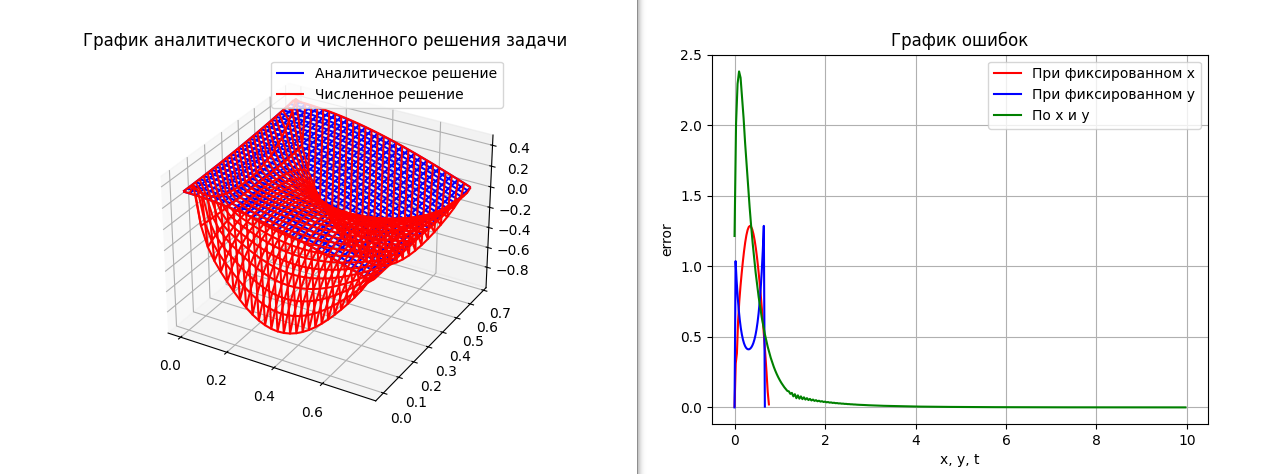
\includegraphics[scale=0.4]{errors.png}
\\

\subsection*{Вывод}

В ходе выполнения лабораторной работы была решена начально-краевая задача для дифференциального уравнения параболического типа. В процессе были получены численные решения, 
для которых последующим шагом была проведена оценка погрешностей. Сравнение численных решений с аналитическими показало, что использованные методы и алгоритмы обладают 
достаточной точностью для рассматриваемых условий задачи. Оценка ошибок позволила подтвердить сходимость и эффективность выбранного численного метода.
\end{document}